\documentclass[11pt,a4paper]{article}

% --- Packages ---
\usepackage[utf8]{inputenc}
\usepackage[margin=1in]{geometry}
\usepackage{amsmath,amssymb}
\usepackage{graphicx}
\usepackage{booktabs}
\usepackage{listings}
\usepackage{xcolor}
\usepackage{fancyhdr}
\usepackage{microtype}
\usepackage{tikz}
\usetikzlibrary{arrows.meta, positioning, shapes.geometric, calc}

% --- Hyperref Setup ---
\usepackage{hyperref}
\hypersetup{
    colorlinks=true,
    linkcolor=blue,
    citecolor=red,
    urlcolor=teal,
    pdftitle={MeetFlow - High-Level Design (HLD)},
    pdfauthor={MeetFlow Engineering Team}
}
\usepackage{cleveref}

% --- Custom Page Layout ---
\pagestyle{fancy}
\fancyhf{}
\setlength{\headheight}{14.5pt}
\rhead{\textbf{MeetFlow HLD}}
\lhead{Browser-to-Browser Video Conferencing}
\rfoot{Page \thepage}
\lfoot{Confidential - For Internal Use Only}
\renewcommand{\headrulewidth}{0.4pt}
\renewcommand{\footrulewidth}{0.4pt}

% --- Code Block Style ---
\definecolor{codegray}{rgb}{0.96,0.96,0.96}
\definecolor{codeblue}{rgb}{0.1,0.2,0.6}
\definecolor{codegreen}{rgb}{0.1,0.5,0.1}

\lstset{
    backgroundcolor=\color{codegray},
    basicstyle=\small\ttfamily,
    breakatwhitespace=false,
    breaklines=true,
    captionpos=b,
    commentstyle=\color{codegreen},
    keywordstyle=\color{codeblue},
    numbers=left,
    numberstyle=\tiny\color{gray},
    numbersep=5pt,
    showspaces=false,
    showstringspaces=false,
    showtabs=false,
    tabsize=2,
    frame=single,
    rulecolor=\color{lightgray}
}

\lstdefinelanguage{json}{
    stringstyle=\color{codeblue},
    string=[s]{"}{"},
    comment=[l]{//},
    morecomment=[s]{/*}{*/},
}

% --- Document Info ---
\title{
    \vspace{2in}
    \Huge \textbf{MeetFlow} \\
    \Large Browser-to-Browser Video Conferencing Application \\
    \vspace{0.5in}
    \huge \textbf{High-Level Design (HLD)}
    \vspace{1.5in}
}
\author{
    \textbf{MeetFlow Engineering Team}
}
\date{June 21, 2026}

\begin{document}

\maketitle
\thispagestyle{empty}
\newpage

\tableofcontents
\newpage

% =========================================================================
\section{Introduction}
% =========================================================================

\subsection{Project Objective}
The objective of the \textbf{MeetFlow} project is to design and develop a secure, robust, and highly responsive browser-based real-time communication platform. MeetFlow allows users to create and join meetings, communicating seamlessly via high-definition video, audio, text chat, screen sharing, and peer-to-peer file transfer. Crucially, the platform operates purely inside modern web browsers without requiring external plugins or native desktop installations.

\subsection{Scope of the Document}
This High-Level Design (HLD) document outlines the architectural blueprint, data models, signaling protocols, and component relationships for MeetFlow. It details how WebRTC, Socket.IO, Node.js, and MySQL combine to support a secure, responsive application.

\subsection{Release Phasing}
To manage complexity and iterate effectively, the application is divided into three major milestones:
\begin{itemize}
    \item \textbf{Phase 1 (One-to-One Baseline):} Direct browser-to-browser audio/video streams, meeting room creation and joining, basic signaling structure.
    \item \textbf{Phase 2 (Collaboration Features):} Real-time text chat, file transfers (via WebRTC Data Channels), screen sharing, and participant roster controls.
    \item \textbf{Phase 3 (Production Readiness):} Database persistence, user account registration/login, JWT authentication, STUN/TURN (Coturn) integration, multi-party SFU topology research, and deployment configurations.
\end{itemize}

% =========================================================================
\section{System Architecture}
% =========================================================================

MeetFlow relies on a hybrid architectural topology. While signaling, user administration, and metadata transactions use a centralized Client-Server model, media streams (audio, video, files) are transmitted directly between browsers using WebRTC's peer-to-peer (P2P) connections.

\subsection{Architectural Components}
The system comprises the following primary building blocks:
\begin{enumerate}
    \item \textbf{Frontend Application (React \& Vite):} A responsive single-page application (SPA) rendering UI panels, requesting camera/microphone access via the browser WebRTC API, and handling peer connection negotiations.
    \item \textbf{Backend Web Server (Node.js \& Express):} Exposes RESTful APIs for user management, authentication, and meeting space configurations.
    \item \textbf{Signaling Server (Socket.IO):} A stateful WebSocket-based messaging node facilitating the initial exchange of session descriptors (SDP) and Network ICE candidates.
    \item \textbf{Database (MySQL):} Stores relational credentials, profiles, meeting logs, and structural data.
    \item \textbf{STUN/TURN Servers (Coturn):} Provides NAT traversal capabilities. STUN identifies public IPs, while TURN acts as a media relay for users behind strict symmetric firewalls.
\end{enumerate}

\subsection{System Architecture Diagram}
\begin{figure}[h!]
\centering
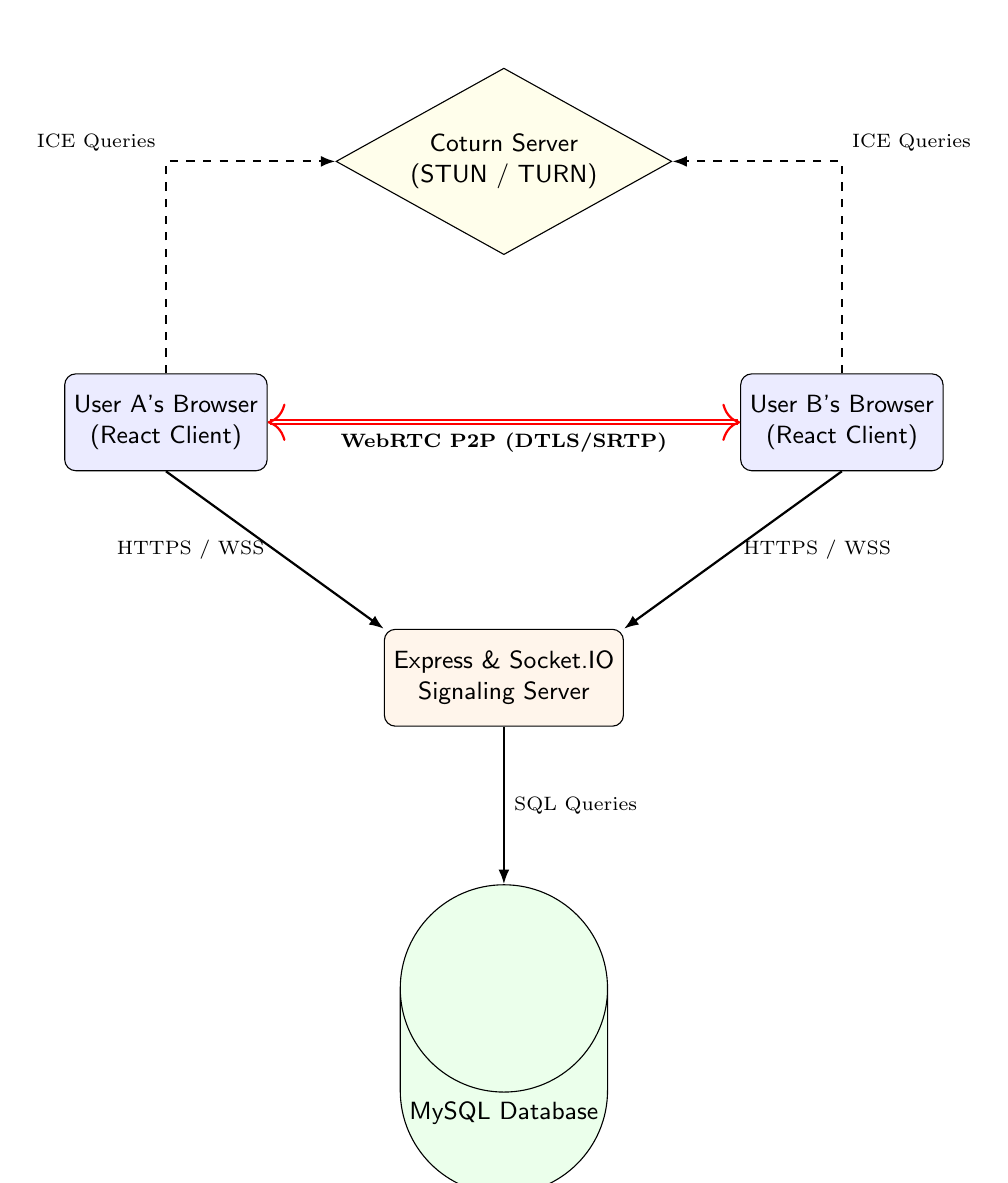
\begin{tikzpicture}[
    node distance=2cm and 2.5cm,
    box/.style={draw, fill=blue!8, rectangle, minimum height=3.5em, minimum width=7em, rounded corners, align=center, font=\small\sffamily},
    db/.style={draw, fill=green!8, cylinder, shape border rotate=90, minimum height=3.5em, minimum width=5em, align=center, font=\small\sffamily},
    server/.style={draw, fill=orange!8, rectangle, minimum height=3.5em, minimum width=8em, rounded corners, align=center, font=\small\sffamily},
    relay/.style={draw, fill=yellow!8, diamond, aspect=1.8, minimum width=6em, align=center, font=\small\sffamily},
    line/.style={draw, -{Latex[scale=0.8]}, thick},
    dashedline/.style={draw, dashed, -{Latex[scale=0.8]}, thick}
]

    % Nodes
    \node[box] (userA) {User A's Browser\\(React Client)};
    \node[box, right=6cm of userA] (userB) {User B's Browser\\(React Client)};
    \node[server, below=2cm of $(userA.south)!0.5!(userB.south)$] (sigServer) {Express \& Socket.IO\\Signaling Server};
    \node[db, below=2cm of sigServer] (mysql) {MySQL Database};
    \node[relay, above=1.5cm of $(userA.north)!0.5!(userB.north)$] (turn) {Coturn Server\\(STUN / TURN)};

    % Lines
    \draw[line] (userA.south) -- (sigServer.north west) node[midway, left, font=\scriptsize] {HTTPS / WSS};
    \draw[line] (userB.south) -- (sigServer.north east) node[midway, right, font=\scriptsize] {HTTPS / WSS};
    \draw[line] (sigServer) -- (mysql) node[midway, right, font=\scriptsize] {SQL Queries};
    
    % STUN/TURN lines
    \draw[dashedline] (userA.north) |- (turn.west) node[midway, above left, font=\scriptsize] {ICE Queries};
    \draw[dashedline] (userB.north) |- (turn.east) node[midway, above right, font=\scriptsize] {ICE Queries};
    
    % P2P Media Connection
    \draw[line, double, <->, red] (userA) -- (userB) node[midway, below, font=\scriptsize\bfseries, color=black] {WebRTC P2P (DTLS/SRTP)};

\end{tikzpicture}
\caption{MeetFlow High-Level Architecture Overview}
\label{fig:sys_architecture}
\end{figure}

\newpage

% =========================================================================
\section{WebRTC Signaling \& Connection Flow}
% =========================================================================

Before User A and User B can streams media directly, they must undergo the signaling phase. The signaling server acts as a post-office, forwarding SDP offers, SDP answers, and ICE Candidates.

\subsection{Signaling Sequence}
The exact steps required to instantiate a peer-to-peer session are detailed below:
\begin{enumerate}
    \item \textbf{Room Entry:} User A joins a meeting room by issuing a \texttt{join-room} event.
    \item \textbf{Discovery:} When User B enters, the signaling server triggers a user-connected notification to User A.
    \item \textbf{Offer Creation:} User A creates a Local Session Description Protocol (SDP) offer containing codec information, media attributes, and cryptographic parameters, and sends it to the Signaling Server.
    \item \textbf{Offer Relay:} The Signaling Server routes the SDP offer directly to User B.
    \item \textbf{Answer Creation:} User B registers User A's offer as its remote description, requests its local audio/video streams, generates an SDP answer, and routes it back through the Signaling Server.
    \item \textbf{Answer Relay:} The Signaling Server forwards the SDP answer to User A.
    \item \textbf{ICE Exchange:} As User A and B discover network pathways (via STUN/TURN queries), they stream their network configurations (\texttt{ice-candidate} events) through the Signaling Server to each other.
    \item \textbf{P2P Connection:} Once descriptions are applied and at least one ICE path is validated, the WebRTC peer connection shifts to the connected state, and direct media streaming commences.
\end{enumerate}

\subsection{Signaling Sequence Diagram}
\begin{figure}[h!]
\centering
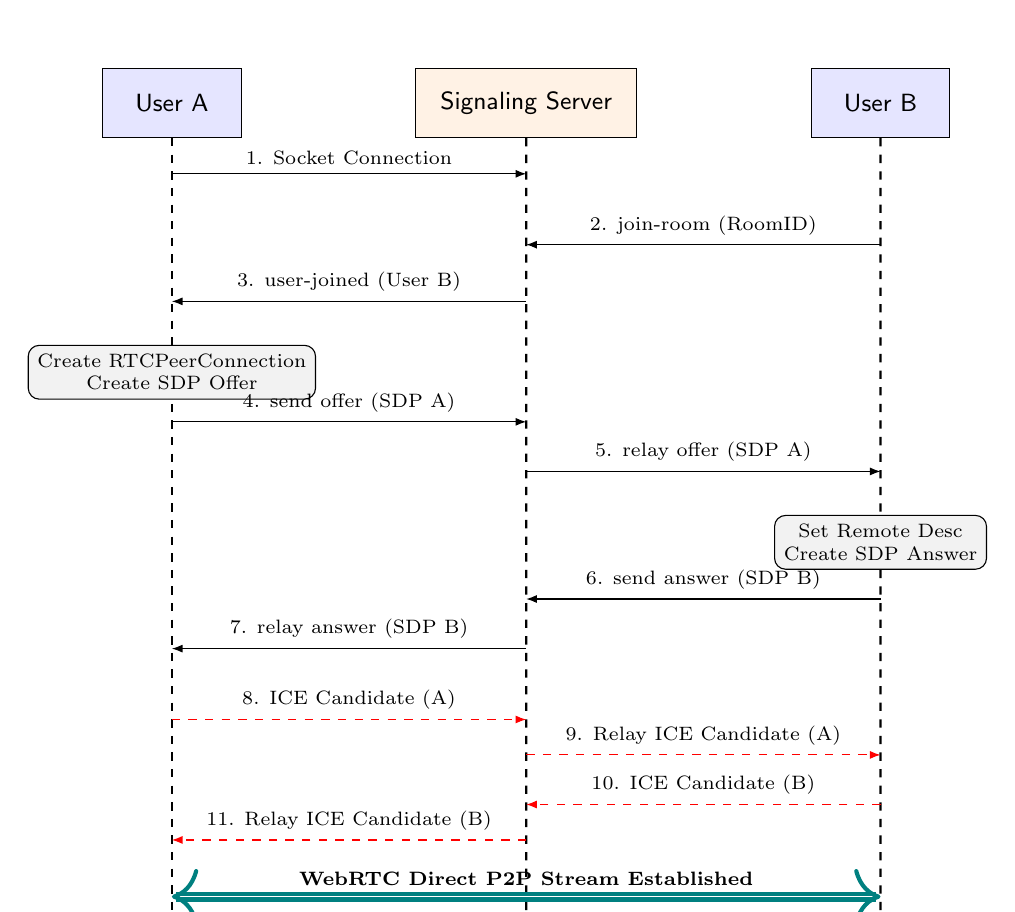
\begin{tikzpicture}[
    scale=0.9,
    every node/.style={font=\small\sffamily},
    actor/.style={draw, fill=blue!10, rectangle, minimum height=2.5em, minimum width=5em, align=center},
    server/.style={draw, fill=orange!10, rectangle, minimum height=2.5em, minimum width=8em, align=center}
]

    % Lifelines
    \node[actor] (A) at (0, 0) {User A};
    \node[server] (S) at (5, 0) {Signaling Server};
    \node[actor] (B) at (10, 0) {User B};
    
    \draw[dashed, thick] (A) -- (0, -11.5);
    \draw[dashed, thick] (S) -- (5, -11.5);
    \draw[dashed, thick] (B) -- (10, -11.5);

    % Steps
    \draw[-{Latex[scale=0.8]}] (0, -1) -- (5, -1) node[midway, above, font=\scriptsize] {1. Socket Connection};
    \draw[-{Latex[scale=0.8]}] (10, -2) -- (5, -2) node[midway, above, font=\scriptsize] {2. join-room (RoomID)};
    \draw[-{Latex[scale=0.8]}] (5, -2.8) -- (0, -2.8) node[midway, above, font=\scriptsize] {3. user-joined (User B)};
    
    \node[align=center, fill=gray!10, draw, font=\scriptsize, rounded corners] at (0, -3.8) {Create RTCPeerConnection\\Create SDP Offer};
    \draw[-{Latex[scale=0.8]}] (0, -4.5) -- (5, -4.5) node[midway, above, font=\scriptsize] {4. send offer (SDP A)};
    \draw[-{Latex[scale=0.8]}] (5, -5.2) -- (10, -5.2) node[midway, above, font=\scriptsize] {5. relay offer (SDP A)};
    
    \node[align=center, fill=gray!10, draw, font=\scriptsize, rounded corners] at (10, -6.2) {Set Remote Desc\\Create SDP Answer};
    \draw[-{Latex[scale=0.8]}] (10, -7.0) -- (5, -7.0) node[midway, above, font=\scriptsize] {6. send answer (SDP B)};
    \draw[-{Latex[scale=0.8]}] (5, -7.7) -- (0, -7.7) node[midway, above, font=\scriptsize] {7. relay answer (SDP B)};
    
    \draw[-{Latex[scale=0.8]}, dashed, color=red] (0, -8.7) -- (5, -8.7) node[midway, above, font=\scriptsize, color=black] {8. ICE Candidate (A)};
    \draw[-{Latex[scale=0.8]}, dashed, color=red] (5, -9.2) -- (10, -9.2) node[midway, above, font=\scriptsize, color=black] {9. Relay ICE Candidate (A)};
    
    \draw[-{Latex[scale=0.8]}, dashed, color=red] (10, -9.9) -- (5, -9.9) node[midway, above, font=\scriptsize, color=black] {10. ICE Candidate (B)};
    \draw[-{Latex[scale=0.8]}, dashed, color=red] (5, -10.4) -- (0, -10.4) node[midway, above, font=\scriptsize, color=black] {11. Relay ICE Candidate (B)};

    \draw[<->, double, color=teal, line width=1.5pt] (0, -11.2) -- (10, -11.2) node[midway, above, font=\scriptsize\bfseries, color=black] {WebRTC Direct P2P Stream Established};

\end{tikzpicture}
\caption{Signaling Protocol Sequence Flow}
\label{fig:sig_sequence}
\end{figure}

\newpage

% =========================================================================
\section{Data Model \& Database Design}
% =========================================================================

MeetFlow relies on a relational database system (MySQL) to maintain user states, profiles, audit records, and history logging.

\subsection{Entity-Relationship Model (Conceptual)}
The core Entities are:
\begin{itemize}
    \item \textbf{User}: Holds basic identification, security hashes, and settings.
    \item \textbf{Meeting}: Tracks unique physical session identifier, creator metadata, active status, and timestamp limits.
    \item \textbf{ParticipantSession}: Intermediary join table auditing which users joined what meeting and at what times.
    \item \textbf{ChatMessage}: Logs text logs sent inside room contexts.
\end{itemize}

\subsection{Database Schema Definitions}

\subsubsection{Users Table}
Tracks registration details and authorization criteria.
\begin{table}[h!]
\centering
\begin{tabular}{@{}llll@{}}
\toprule
\textbf{Column Name} & \textbf{Data Type} & \textbf{Attributes} & \textbf{Description} \\ \midrule
\texttt{id} & INT & PK, AUTO\_INCREMENT & Unique identifier for the user. \\
\texttt{username} & VARCHAR(50) & UNIQUE, NOT NULL & User-selected screen handle. \\
\texttt{email} & VARCHAR(100) & UNIQUE, NOT NULL & Verified user email address. \\
\texttt{password\_hash} & VARCHAR(255) & NOT NULL & Bcrypt password digest. \\
\texttt{avatar\_url} & VARCHAR(255) & NULL & URI locating user's custom profile picture. \\
\texttt{created\_at} & TIMESTAMP & DEFAULT CURRENT\_TIMESTAMP & Date of account generation. \\
\texttt{updated\_at} & TIMESTAMP & ON UPDATE CURRENT\_TIMESTAMP & Date of last profile alteration. \\ \bottomrule
\end{tabular}
\caption{Users Table Schema}
\label{tab:users_table}
\end{table}

\subsubsection{Meetings Table}
Tracks unique session tokens and runtime status.
\begin{table}[h!]
\centering
\begin{tabular}{@{}llll@{}}
\toprule
\textbf{Column Name} & \textbf{Data Type} & \textbf{Attributes} & \textbf{Description} \\ \midrule
\texttt{id} & VARCHAR(12) & PK & Unique URL identifier (e.g., \texttt{ABCD-EFGH}). \\
\texttt{host\_id} & INT & FK (users.id) & Identifies the user who initiated the meeting. \\
\texttt{created\_at} & TIMESTAMP & DEFAULT CURRENT\_TIMESTAMP & Start timestamp of the session. \\
\texttt{ended\_at} & TIMESTAMP & NULL & Termination timestamp of the session. \\
\texttt{status} & ENUM & ('active', 'ended') & Current execution state of the room. \\ \bottomrule
\end{tabular}
\caption{Meetings Table Schema}
\label{tab:meetings_table}
\end{table}

\subsubsection{Meeting\_Participants Table}
Audits individual attendees for analytics and history display.
\begin{table}[h!]
\centering
\begin{tabular}{@{}llll@{}}
\toprule
\textbf{Column Name} & \textbf{Data Type} & \textbf{Attributes} & \textbf{Description} \\ \midrule
\texttt{id} & INT & PK, AUTO\_INCREMENT & Unique row ID. \\
\texttt{meeting\_id} & VARCHAR(12) & FK (meetings.id), NOT NULL & Target meeting room. \\
\texttt{user\_id} & INT & FK (users.id), NOT NULL & Participating member. \\
\texttt{joined\_at} & TIMESTAMP & DEFAULT CURRENT\_TIMESTAMP & Entrance timestamp. \\
\texttt{left\_at} & TIMESTAMP & NULL & Leaving timestamp. \\ \bottomrule
\end{tabular}
\caption{Meeting Participants Table Schema}
\label{tab:participants_table}
\end{table}

\newpage

% =========================================================================
\section{API \& WebSocket Interface Specifications}
% =========================================================================

\subsection{RESTful Web APIs}

\subsubsection{User Registration}
\begin{itemize}
    \item \textbf{Endpoint:} \texttt{POST /api/auth/register}
    \item \textbf{Description:} Creates a new user record.
    \item \textbf{Request Payload:}
\begin{lstlisting}[language=json]
{
  "username": "johndoe",
  "email": "johndoe@example.com",
  "password": "SecurePassword123!"
}
\end{lstlisting}
    \item \textbf{Response Payload (Success 201 Created):}
\begin{lstlisting}[language=json]
{
  "message": "User registered successfully",
  "userId": 101
}
\end{lstlisting}
\end{itemize}

\subsubsection{User Login}
\begin{itemize}
    \item \textbf{Endpoint:} \texttt{POST /api/auth/login}
    \item \textbf{Description:} Validates credentials and returns a JWT.
    \item \textbf{Request Payload:}
\begin{lstlisting}[language=json]
{
  "email": "johndoe@example.com",
  "password": "SecurePassword123!"
}
\end{lstlisting}
    \item \textbf{Response Payload (Success 200 OK):}
\begin{lstlisting}[language=json]
{
  "token": "eyJhbGciOiJIUzI1NiIsInR5cCI6IkpXVCJ9...",
  "user": {
    "id": 101,
    "username": "johndoe",
    "email": "johndoe@example.com",
    "avatarUrl": null
  }
}
\end{lstlisting}
\end{itemize}

\subsubsection{Create Meeting}
\begin{itemize}
    \item \textbf{Endpoint:} \texttt{POST /api/meeting/create}
    \item \textbf{Description:} Instantiates an active meeting record. Requires authorization header: \texttt{Authorization: Bearer <token>}.
    \item \textbf{Response Payload (Success 200 OK):}
\begin{lstlisting}[language=json]
{
  "meetingId": "ABCD-EFGH",
  "hostId": 101,
  "createdAt": "2026-06-21T22:58:55.000Z"
}
\end{lstlisting}
\end{itemize}

\subsection{WebSocket Signaling Events}
These events are transmitted using Socket.IO during an active video conference.

\begin{itemize}
    \item \textbf{\texttt{join-room} (Client $\rightarrow$ Server):} Initiated when the client navigates into a room.
\begin{lstlisting}[language=json]
{
  "roomId": "ABCD-EFGH",
  "userId": 101,
  "username": "johndoe"
}
\end{lstlisting}
    \item \textbf{\texttt{offer} (Client $\rightarrow$ Server $\rightarrow$ Target Client):} Transmits the local SDP offer.
\begin{lstlisting}[language=json]
{
  "targetSocketId": "socket_id_of_recipient",
  "offer": {
    "type": "offer",
    "sdp": "v=0\r\no=alice 2890844526..."
  }
}
\end{lstlisting}
    \item \textbf{\texttt{answer} (Client $\rightarrow$ Server $\rightarrow$ Target Client):} Relays the SDP answer.
\begin{lstlisting}[language=json]
{
  "targetSocketId": "socket_id_of_recipient",
  "answer": {
    "type": "answer",
    "sdp": "v=0\r\no=bob 2890844527..."
  }
}
\end{lstlisting}
    \item \textbf{\texttt{ice-candidate} (Client $\rightarrow$ Server $\rightarrow$ Target Client):} Streams discovered ICE pathways.
\begin{lstlisting}[language=json]
{
  "targetSocketId": "socket_id_of_recipient",
  "candidate": {
    "candidate": "candidate:842163049 1 udp 1686052607 192.168.1.2 55301 typ host...",
    "sdpMid": "0",
    "sdpMLineIndex": 0
  }
}
\end{lstlisting}
\end{itemize}

% =========================================================================
\section{Security, Performance \& Reliability}
% =========================================================================

\subsection{Security Engineering}
Security is a foundational tenet of MeetFlow's real-time communication stack.
\begin{itemize}
    \item \textbf{Transport Security:} All traffic (HTTPS, WSS) is encrypted using Transport Layer Security (TLS 1.3) to prevent eavesdropping and hijacking.
    \item \textbf{Media Encryption:} WebRTC enforces mandatory end-to-end media encryption. Signaling channels exchange temporary cryptographic keys, and the media streams are secured using \textbf{DTLS} (Datagram Transport Layer Security) and \textbf{SRTP} (Secure Real-time Transport Protocol).
    \item \textbf{JWT Authentication:} RESTful API commands targeting meeting configurations require validating cryptographically signed JSON Web Tokens.
    \item \textbf{Credential Protection:} Password assets are hashed using the CPU-bound \textbf{Bcrypt} framework utilizing an index work factor of 12.
\end{itemize}

\subsection{Performance Goals}
\begin{itemize}
    \item \textbf{Session Setup Latency:} Mean duration to transition from room ID entry to video visibility must remain lower than $5$ seconds under normal network conditions.
    \item \textbf{Real-Time Network Latency:} One-way end-to-end media latency must stay below $200$\,ms. Jitter buffers adjust dynamically to smooth out stream variance.
    \item \textbf{Resolution \& Bandwidth Adaptation:} Client implementations utilize \texttt{RTCRtpSender.setParameters()} or WebRTC's default simulcast capability to lower output resolutions dynamically based on local congestion detections.
\end{itemize}

\subsection{Reliability and Fault Tolerance}
\begin{itemize}
    \item \textbf{Automatic Reconnection:} If the signaling WebSocket connection drops, Socket.IO is configured to execute exponential back-off reconnections.
    \item \textbf{ICE Restart:} If network changes occur (e.g., switching from Wi-Fi to cellular data), the client initiates a WebRTC ICE restart procedure, triggering a fresh offer-answer exchange over the active signaling channel.
\end{itemize}

\newpage

% =========================================================================
\section{User Interface \& Meeting Layout}
% =========================================================================

\subsection{UI Pages Map}
The web app is structured into pages detailed in the hierarchy below:
\begin{itemize}
    \item \textbf{Landing Home Page:} Explains features with direct buttons to register or log in.
    \item \textbf{Dashboard:} Displays upcoming meetings, meeting history, profiles access, and a simple box to ``Start Meeting'' or ``Join Meeting''.
    \item \textbf{Meeting Room Screen:} The unified workspace where real-time video grid and utility sidebars render.
\end{itemize}

\subsection{Meeting Room Design Grid Layout}
The structural configuration of the meeting page is diagrammed below:

\begin{figure}[h!]
\centering
\begin{minipage}{0.9\textwidth}
\begin{verbatim}
+-----------------------------------------------------------------------+
|  MeetFlow                                                             |
+----------------------------------------------------+------------------+
|                                                    |                  |
|                                                    |                  |
|                    Local Video                     |    Chat Panel    |
|                                                    |                  |
|                                                    |                  |
|                                                    |  [User A] Hello! |
|                                                    |  [User B] Hi!    |
|                                                    |                  |
+----------------------------------------------------+                  |
|                                                    |                  |
|                                                    |                  |
|                    Remote Video                    |                  |
|                                                    |                  |
|                                                    |                  |
|                                                    |                  |
|                                                    | [Send Message  ] |
+----------------------------------------------------+------------------+
|  [Mic]  [Cam]  [Share]  [Chat]  [Users]  [File]            [Leave]    |
+-----------------------------------------------------------------------+
\end{verbatim}
\end{minipage}
\caption{Visual Mockup Grid of the Meeting Room Screen}
\label{fig:ui_grid}
\end{figure}

The layout comprises three distinct flex zones:
\begin{enumerate}
    \item \textbf{Media Stage (Left Area):} Displays the feed of the local user and the incoming feed of the remote participant in a grid.
    \item \textbf{Sidebar (Right Area):} Toggles dynamically between the Chat log and the active Participants list.
    \item \textbf{Control Deck (Bottom Bar):} A floating, glassmorphic HUD bar exposing mute/unmute buttons, camera toggles, screen sharing buttons, file uploads, chat toggle, and a leave meeting button.
\end{enumerate}

\end{document}
